\documentclass[11pt]{article}
\usepackage{a4wide}
%\raggedright
%\usepackage{driverbook}
\usepackage{latexsym}           % math symbols that were omitted in latex2e
\usepackage{amsbsy}             % bold greek defs
\usepackage{amsmath,graphicx}
\usepackage{bbm}
\usepackage{mathrsfs}
\usepackage{stmaryrd}
\usepackage{graphics}
\usepackage{acronym}
\usepackage{longtable}
\usepackage{mathtools}
\usepackage{times}
\usepackage{setspace}
\usepackage{cite}
\usepackage{array}
\usepackage{subfigure}
\usepackage{amsmath,amsthm}
\usepackage{amssymb}
\usepackage{wasysym,url}
\usepackage{fixltx2e,amsmath}
\usepackage{setspace,float}
\usepackage{color}
\usepackage{cases,bm}
\usepackage{mathrsfs}
\usepackage{enumitem}
\usepackage{hyperref}
\usepackage{mathtools,cuted}
\usepackage[linesnumbered,ruled,vlined]{algorithm2e}
\usepackage{epsfig}
\usepackage{color}
\DontPrintSemicolon

\usepackage{geometry}
 \geometry{
 a4paper,
 total={170mm,257mm},
 left=20mm,
 top=30mm,
 bottom=30mm,
 }
 
 
\usepackage{listings}
\usepackage{xcolor}

\definecolor{codegreen}{rgb}{0,0.6,0}
\definecolor{codegray}{rgb}{0.5,0.5,0.5}
\definecolor{codepurple}{rgb}{0.58,0,0.82}
\definecolor{backcolour}{rgb}{0.95,0.95,0.92}

\lstdefinestyle{mystyle}{
    backgroundcolor=\color{backcolour},   
    commentstyle=\color{codegreen},
    keywordstyle=\color{magenta},
    numberstyle=\tiny\color{codegray},
    stringstyle=\color{codepurple},
    basicstyle=\ttfamily\footnotesize,
    breakatwhitespace=false,         
    breaklines=true,                 
    captionpos=b,                    
    keepspaces=true,                 
    numbers=left,                    
    numbersep=5pt,                  
    showspaces=false,                
    showstringspaces=false,
    showtabs=false,                  
    tabsize=2
}

\lstset{style=mystyle}

\newcommand{\by}{\mathbf{y}}
\newcommand{\br}{\mathbf{r}}
\newcommand{\bd}{\mathbf{d}}
\newcommand{\bn}{\mathbf{n}}
\newcommand{\bh}{\mathbf{h}}
\newcommand{\bx}{\mathbf{x}}
\newcommand{\be}{\mathbf{e}}
\newcommand{\bw}{\mathbf{w}}
\newcommand{\bW}{\mathbf{W}}
\newcommand{\bI}{\mathbf{I}}
\newcommand{\bA}{\mathbf{A}}
\newcommand{\bH}{\mathbf{H}}
\newcommand{\bQ}{\mathbf{Q}}
\newcommand{\bG}{\mathbf{G}}
\newcommand{\bC}{\mathbf{C}}
\newcommand{\rr}{\mathbb{R}}
\newcommand{\zz}{\mathbb{Z}}
\newcommand{\nn}{\mathbb{N}}
\newcommand{\cc}{\mathbb{C}}
\newcommand{\Ex}{\mathbb{E}}
\newcommand{\TT}{\mathsf{T}}
\newcommand{\HH}{\mathsf{H}}
\newcommand{\dd}{\mathrm{d}}
\newcommand{\jj}{\mathrm{j}}

\newcommand{\zerovec}{\boldsymbol{0}}
\newcommand{\bSigma}{\boldsymbol{\Sigma}}
\newcommand{\btheta}{\boldsymbol{\theta}}
\newcommand{\bgamma}{\boldsymbol{\gamma}}

\begin{document}
\thispagestyle{empty}

{\small
\begin{flushleft}
   Name: Abijith J. Kamath\\
   Student Id: 17788
\end{flushleft}
}
\vspace{2ex}
\begin{center}
    {\Large\bf E1 244: Detection and Estimation}\\
    February-May 2021

\vspace{5mm}
{\bf Solution -- Homework 1}
\end{center}
\vspace{5mm}

\section*{Analysis and Algorithms for Time-Difference-of-Arrival (TDOA) Localisation}

% -----------------------------------------------------------------------------------------------------------------------
% -----------------------------------------------------------------------------------------------------------------------

\subsection*{Part A: Derivation and Modelling}
\label{subsec:partA}

Let the 2D position of the target be $\bx = [x \; y]^{\TT}$, and let $\{\bx_{i}\}_{i=1}^{M}$ be the position of the $M$ sensors used to locate the target. The TDOA system measures difference in ranges using the time-delay of a test signal and the measurements are modelled as:
\begin{equation}
	r_{i} = cT_{0} + d_{i} + w_{i}, \; i=1,\cdots,M,
\label{eq:signalModel}
\end{equation}
where $T_{0}$ is the time at which the target emits the beacon, $c$ is the speed of propagation of the wave, $d_{i} = \Vert \bx-\bx_{i} \Vert_{2}$ is the distance between the sensors and the target and $w_{i}$ is additive white Gaussian noise with uniform variance $\sigma^{2}$. In the case of this example, the number of sensors $M=4$. In TDOA, to eliminate $T_{0}$, the difference in the ranges is used, i.e.,
\begin{equation}
	r_{ij} = d_{i} - d_{j} + n_{ij}, \; i,j=1,2,3,4,
\label{eq:measurementModel}
\end{equation}
where $n_{ij} = w_{i}-w_{j}$. The differences in ranges are used for estimation of the unknown location of the target $\bx$. \\

To estimate the 2D position of the target, three range measurements are sufficient. This implies three range-difference measurements are sufficient. We consider the following measurements for estimation:
\begin{equation}
	\underbrace{\begin{bmatrix}
		r_{12} \\ r_{23} \\ r_{34}
	\end{bmatrix}}_{\br} = 
	\underbrace{\begin{bmatrix}
		d_{1}-d_{2} \\ d_{2}-d_{3} \\ d_{3}-d_{4}
	\end{bmatrix}}_{\bd(\bx)} +
	\underbrace{\begin{bmatrix}
		n_{12} \\ n_{23} \\ n_{34}
	\end{bmatrix}}_{\bn}.
\label{eq:estimationModel}
\end{equation}
The noise $\bn$ in (\ref{eq:estimationModel}) is a linear transformation of the i.i.d Gaussian random vector with zero mean and variance $\sigma^{2}$. The transformation is given by:
\begin{equation}
	\bn = \begin{bmatrix}
		w_{1} - w_{2} \\ w_{2} - w_{3} \\ w_{3} - w_{4}
	\end{bmatrix} = 
	\underbrace{\begin{bmatrix}
		1 & -1 & 0 & 0 \\
		0 & 1 & -1 & 0 \\
		0 & 0 & 1 & -1 \\
	\end{bmatrix}}_{\bA}
	\begin{bmatrix}
		w_{1} \\ w_{2} \\ w_{3} \\ w_{4}
	\end{bmatrix}.
\label{eq:noiseModel}
\end{equation}
Therefore, distribution of $\bn$ is Gaussian with mean $\Ex \left[ \bn \right] = \bA \Ex \left[ \bw \right] = \zerovec$, and covariance matrix $\bSigma = \Ex \left[ \bn \bn^{\TT} \right] = \bA \Ex \left[ \bw \bw^{\TT} \right] \bA = \sigma^{2} \bA \bA^{\TT}$. Therefore, the joint data-distribution of the measurements $\br$ is also Gaussian, i.e., $\br \sim \mathcal{N} \left( \bd(\bx), \bSigma \right)$.

% -----------------------------------------------------------------------------------------------------------------------

\subsubsection*{Derivation of Cram\'er-Rao Lower Bound}
\label{subsubsec:crlb}

The likelihood function using the joint data-distribution:
\begin{equation}
\begin{split}
	p(\br ; \bx) &= \frac{1}{(2\pi)^{3/2} (\det \bSigma)^{1/2}} \mathrm{exp} \left( -\frac{1}{2} (\br - \bd(\bx))^{\TT} \bSigma^{-1} (\br - \bd(\bx)) \right), \\
	\implies \ln p(\br ; \bx) &= -\frac{3}{2} \ln (2\pi) - \frac{1}{2} \ln \det \bSigma -\frac{1}{2} (\br - \bd(\bx))^{\TT} \bSigma^{-1} (\br - \bd(\bx)),
\end{split}
\label{eq:likelihood}
\end{equation}
and therefore the score function is given by:
\begin{equation}
	\nabla_{\bx} \ln p(\br ; \bx) = - \left( \frac{\partial \bd(\bx)}{\partial \bx} \right)^{\TT} \bSigma^{-1} \left( \br - \bd(\bx) \right).
\label{eq:regularity}
\end{equation}
It can be seen that $\displaystyle \Ex \left[ \nabla_{\bx} \ln p(\br ; \bx) \right] = \zerovec$, i.e., the joint data-distribution satisfies regularity conditions. Therefore, the inverse Fisher information matrix (FIM) gives a lower bound on the covariance of any unbiased estimator for $\bx$. The Fisher information matrix is given by:
\begin{equation}
\begin{split}
	\bI(\bx) &= \Ex \left[ \left( \nabla_{\bx} \ln p(\br ; \bx) \right) \left( \nabla_{\bx} \ln p(\br ; \bx) \right)^{\TT} \right], \\
	&= \Ex \left[ \left( \frac{\partial \bd(\bx)}{\partial \bx} \right)^{\TT} \bSigma^{-1} \left( \br - \bd(\bx) \right) \left( \br - \bd(\bx) \right)^{\TT} \bSigma^{-1} \left( \frac{\partial \bd(\bx)}{\partial \bx} \right) \right], \\
	&= \left( \frac{\partial \bd(\bx)}{\partial \bx} \right)^{\TT} \bSigma^{-1} \underbrace{\Ex \left[ \left( \br - \bd(\bx) \right) \left( \br - \bd(\bx) \right)^{\TT} \right]}_{\bSigma} \bSigma^{-1} \left( \frac{\partial \bd(\bx)}{\partial \bx} \right), \\
	&= \left( \frac{\partial \bd(\bx)}{\partial \bx} \right)^{\TT} \bSigma^{-1} \left( \frac{\partial \bd(\bx)}{\partial \bx} \right),
\end{split}
\label{eq:fim}
\end{equation}
where the derivative $\displaystyle \frac{\partial \bd(\bx)}{\partial \bx}$ is the matrix,
\begin{equation}
	\frac{\partial \bd(\bx)}{\partial \bx} = \begin{bmatrix}
		\frac{\partial}{\partial x} (d_{1} - d_{2}) & \frac{\partial}{\partial y} (d_{1} - d_{2}) \\
		\frac{\partial}{\partial x} (d_{2} - d_{3}) & \frac{\partial}{\partial y} (d_{2} - d_{3}) \\
		\frac{\partial}{\partial x} (d_{3} - d_{4}) & \frac{\partial}{\partial y} (d_{3} - d_{4})
	\end{bmatrix},
\label{eq:derivative}
\end{equation}
and the entries are computed as $\displaystyle \frac{\partial}{\partial x} (d_{i} - d_{j}) = \frac{x-x_{i}}{d_{i}} - \frac{x-x_{j}}{d_{j}}$, and similarly with respect to $y$. Let $\hat{\bx}$ be any unbiased estimator for $\bx$. Then, using Cram\'er-Rao lower bound (CRLB) theorem:
\begin{equation}
	\mathrm{cov}(\hat{\bx}) \geq \bI (\bx)^{-1},
\label{eq:crlb}
\end{equation}
and therefore the variance of the estimates for the coordinates, $\mathrm{var}(\hat{x}) \geq [\bI (\bx)]^{-1}_{11}$ and $\mathrm{var}(\hat{y}) \geq [\bI (\bx)]^{-1}_{22}$.

% -----------------------------------------------------------------------------------------------------------------------

\subsubsection*{Maximum-Likelihood Estimator (MLE)}
\label{subsubsec:mle}

The maximum-likelihood estimator (MLE) for the parameter $\bx$ is given by:
\begin{equation}
\begin{split}
	\hat{\bx}_{MLE} &= \mathrm{arg }\max_{\bx \in \rr^{2}} p(\br ; \bx), \\
	&= \mathrm{arg }\max_{\bx \in \rr^{2}} \ln p(\br ; \bx), \\
	&= \mathrm{arg }\min_{\bx \in \rr^{2}} J(\bx) \doteq \frac{1}{2} (\br - \bd(\bx))^{\TT} \bSigma^{-1} (\br - \bd(\bx)).
\end{split}
\label{eq:mle}
\end{equation}
The MLE is given by the solution to the unconstrained optimisation programme, and we choose gradient descent with fixed step-size to solve the optimisation programme. The gradient descent updates with constant step-size $\alpha > 0$ are given by:
\begin{equation}
\begin{split}
	\hat{\bx}^{(k+1)} &= \hat{\bx}^{(k)} - \alpha \nabla_{\bx} J(\bx^{(k)}), \\
	&= \hat{\bx}^{(k)} + \alpha \left( \frac{\partial \bd(\bx^{(k)})}{\partial \bx} \right)^{\TT} \bSigma^{-1} \left( \br - \bd(\bx^{(k)}) \right),
\end{split}
\label{eq:gradientDescentMLE}
\end{equation}
where the gradient of the objective function is given identical to (\ref{eq:regularity}). The iterations are run until the error between successive updates is below tolerance or the maximum number of iterations is reached. The estimates of the coordinates of the target position from the MLE iterations in (\ref{eq:gradientDescentMLE}) is given directly by the entries of the vector.

% -----------------------------------------------------------------------------------------------------------------------

\subsubsection*{Best-Linear-Unbiased Estimator (BLUE)}
\label{subsubsec:blue}

The linearisation of the range measurements in (\ref{eq:measurementModel}) gives:
\begin{equation}
	r_{ij}^{2} + d_{j}^{2} + 2r_{ij}d_{j} = d_{i}^{2} + e_{ij},
\label{eq:linearModel}
\end{equation}
where the noise is approximates as $e_{ij} = n_{ij}^{2} = (w_{i} - w_{j})^{2}$. Using $d_{i}^{2} = \Vert \bx - \bx_{i} \Vert_{2}^{2}$ in (\ref{eq:linearModel}), we get:
\begin{equation}
	r_{ij}^{2} - \Vert \bx_{i} \Vert_{2}^{2} + \Vert \bx_{j} \Vert_{2}^{2} = -2(\bx_{i} - \bx_{j})^{\TT} \bx - 2r_{ij}d_{j} + e_{ij},
\label{eq:blueSystem}
\end{equation}
which is linear in the parameter $\bx$. In matrix-vector form, and taking the parameter vector $\btheta = [x \; y \; d_{2} \; d_{3} \; d_{4}]^{\TT}$, we have:
\begin{equation}
	\underbrace{\begin{bmatrix}
		r^{2}_{12} - \Vert \bx_{1} \Vert_{2}^{2} + \Vert \bx_{2} \Vert_{2}^{2} \\
		r^{2}_{13} - \Vert \bx_{1} \Vert_{2}^{2} + \Vert \bx_{3} \Vert_{2}^{2} \\
		r^{2}_{14} - \Vert \bx_{1} \Vert_{2}^{2} + \Vert \bx_{4} \Vert_{2}^{2} \\
		r^{2}_{23} - \Vert \bx_{2} \Vert_{2}^{2} + \Vert \bx_{3} \Vert_{2}^{2} \\
		r^{2}_{24} - \Vert \bx_{2} \Vert_{2}^{2} + \Vert \bx_{4} \Vert_{2}^{2} \\
		r^{2}_{34} - \Vert \bx_{3} \Vert_{2}^{2} + \Vert \bx_{4} \Vert_{2}^{2} \\
	\end{bmatrix}}_{\bgamma} = 
	\underbrace{\begin{bmatrix}
		-2(x_{1} - x_{2}) & -2(y_{1} - y_{2}) & -2r_{12} & 0 & 0 \\
		-2(x_{1} - x_{3}) & -2(y_{1} - y_{3}) & 0 & -2r_{13} & 0 \\
		-2(x_{1} - x_{4}) & -2(y_{1} - y_{4}) & 0 & 0 & -2r_{14} \\
		-2(x_{2} - x_{3}) & -2(y_{2} - y_{3}) & 0 & -2r_{23} & 0 \\
		-2(x_{2} - x_{4}) & -2(y_{2} - y_{4}) & 0 & 0 & -2r_{24} \\
		-2(x_{3} - x_{4}) & -2(y_{3} - y_{4}) & 0 & 0 & -2r_{34} \\
	\end{bmatrix}}_{\bH}
	\underbrace{\begin{bmatrix}
		x \\ y \\ d_{2} \\ d_{3} \\ d_{4}
	\end{bmatrix}}_{\btheta} +
	\underbrace{\begin{bmatrix}
		e_{12} \\ e_{13} \\ e_{14} \\ d_{23} \\ e_{24} \\ e_{34}
	\end{bmatrix}}_{\be}.
\label{eq:blueModel}
\end{equation}
The complete distribution of the random vector $\be$ is not important for estimation, and only mean and covariance of the distribution are sufficient. The mean of the entries $\Ex[e_{ij}] = \Ex[(w_{i} - w_{j})^{2}] = \mathrm{var}(w_{i}^{2}) + \mathrm{var}(w_{j}^{2}) = 2\sigma^{2}$. The mean subtracted model $\bgamma - 2\sigma^{2} \mathbbm{1} = \bH\btheta + \bar{\be}$, where $\bar{\be} = \be - 2\sigma^{2}\mathbbm{1}$ is a zero mean random vector, and $\mathbbm{1}$ is the all-ones vector. The covariance matrix of the random vector $\bC = \Ex[\bar{\be}\bar{\be}^{\TT}] = \Ex[\be \be^{\TT}] - 4\sigma^{4} \bI$. The entries are computed as: $[\bC]_{11} = \Ex[(w_{1}-w_{2})^{2})(w_{1}-w_{2})^{2})] - 4\sigma^{4} = 3\sigma^{4} + 3\sigma^{4} + 6\sigma^{4} - 4\sigma^{4} = 8\sigma^{4}$, $[\bC]_{13} = [\bC]_{14} = [\bC]_{15} = \Ex[(w_{1}-w_{2})^{2}(w_{1}-w_{4})^{2}]-4\sigma^{4} = 2\sigma^{4}$, and $[\bC]_{16} = \Ex[(w_{1}-w_{2})^{2}(w_{3}-w_{4})^{2}] = 0$. Similarly, we see that the diagonal entries are all equal to $[\bC]_{11}$ and all the anti-diagonal entries are equal to zero. All other entries are equal to $[\bC]_{12}$. Therefore the covariance matrix is equal to:
\begin{equation}
	\bC = 2\sigma^{4} \begin{bmatrix}
		4 & 1 & 1 & 1 & 1 & 0 \\
		1 & 4 & 1 & 1 & 0 & 1 \\
		1 & 1 & 4 & 0 & 1 & 1 \\
		1 & 1 & 0 & 4 & 1 & 1 \\
		1 & 0 & 1 & 1 & 4 & 1 \\
		0 & 1 & 1 & 1 & 1 & 4 \\
	\end{bmatrix}.
\label{eq:blueCov}
\end{equation}
Then, the BLUE estimate for the parameter vector $\btheta$ is given by $\displaystyle \hat{\btheta} = \left( \bH^{\TT} \bC^{-1}\bH \right)^{-1} \bH^{\TT} \bC^{-1} \left( \bgamma - 2\sigma^{2} \mathbbm{1} \right)$. The estimates of the coordinates of the target position from the BLUE estimate for $\btheta$ is then $\hat{x}_{BLUE} = [\hat{\btheta}]_{1}$ and $\hat{y}_{BLUE} = [\hat{\btheta}]_{2}$.

% -----------------------------------------------------------------------------------------------------------------------
% -----------------------------------------------------------------------------------------------------------------------

\subsection*{Part B: Implementation}
\label{subsec:partB}

% -----------------------------------------------------------------------------------------------------------------------

\subsubsection*{Maximum-Likelihood Estimator (MLE)}
\label{subsubsec:mleImplementation}

Figure \ref{fig:mle} shows the TDOA localisation using MLE. The distance measurements have additive white Gaussian noise with variance $\sigma^{2} = 0.001$. The estimated location of the target $\hat{\bx}_{MLE}$ is exact.

% -----------------------------------------------------------------------------------------------------------------------

\subsubsection*{Best-Linear-Unbiased Estimator (BLUE)}
\label{subsubsec:blueImplementation}

Figure \ref{fig:blue} shows the TDOA localisation using BLUE. The distance measurements have additive white Gaussian noise with variance $\sigma^{2} = 0.001$. The estimated location of the target $\hat{\bx}_{BLUE}$ is exact and overlaps with $\hat{\bx}_{MLE}$.
\begin{figure}[h]
\centering
\subfigure[]{\label{fig:mle}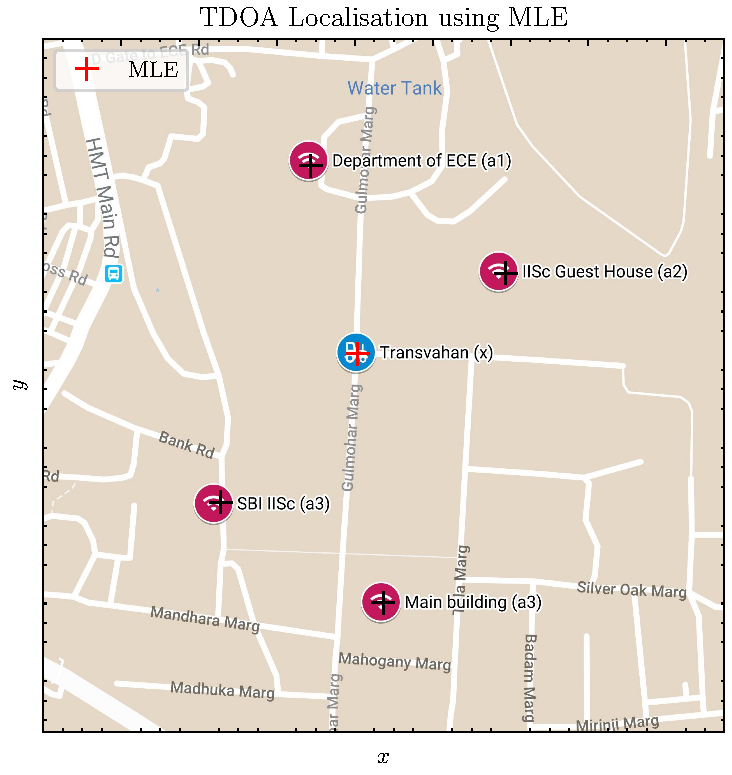
\includegraphics[width=3in]{../results/mle.pdf}}
\subfigure[]{\label{fig:blue}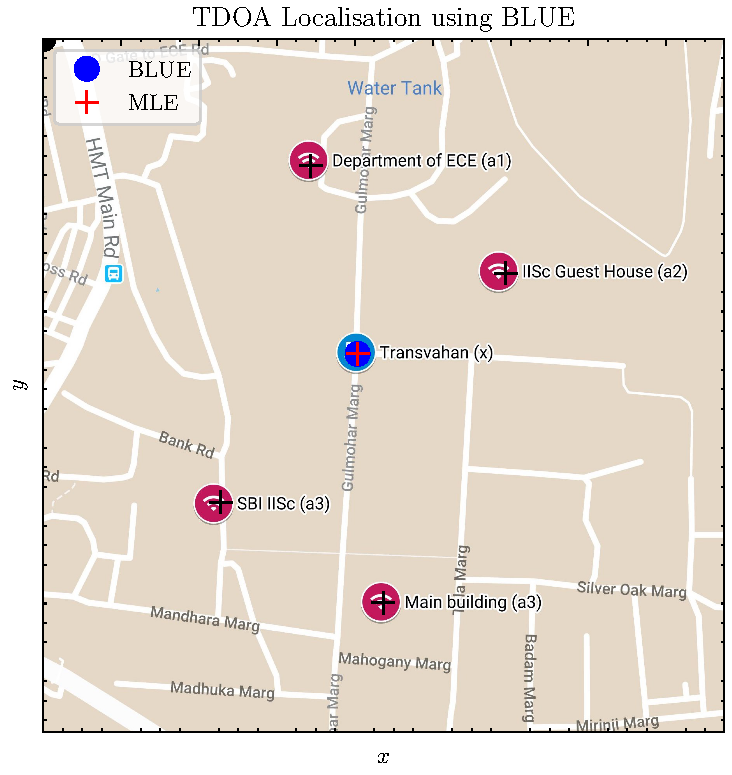
\includegraphics[width=3in]{../results/blue.pdf}}
\caption{TDOA localisation using MLE and BLUE.}
\end{figure}

% -----------------------------------------------------------------------------------------------------------------------

\subsubsection*{Noise Analysis}
\label{subsubsec:noiseAnalysis}

Figure \ref{fig:crlbX} and \ref{fig:crlbY} shows the mean-squared-error (MSE) between estimated target location and true target location for varying values of $\sigma^{2}$, using MLE and BLUE respectively; along with their corresponding CRLB. It can be seen that the MLE and BLUE achieve CRLB as the $
\sigma^{2}$ goes to zero. It can also be observed that the MLE estimate consistently has a lower MSE than the BLUE estimate. Further, the MLE estimate has MSE achieving the CRLB even for higher values of $\sigma^{2}$, whereas the BLUE estimate is evidently suboptimal for higher values of $\sigma^{2}$.
\begin{figure}[t!]
\centering
\subfigure[]{\label{fig:crlbX}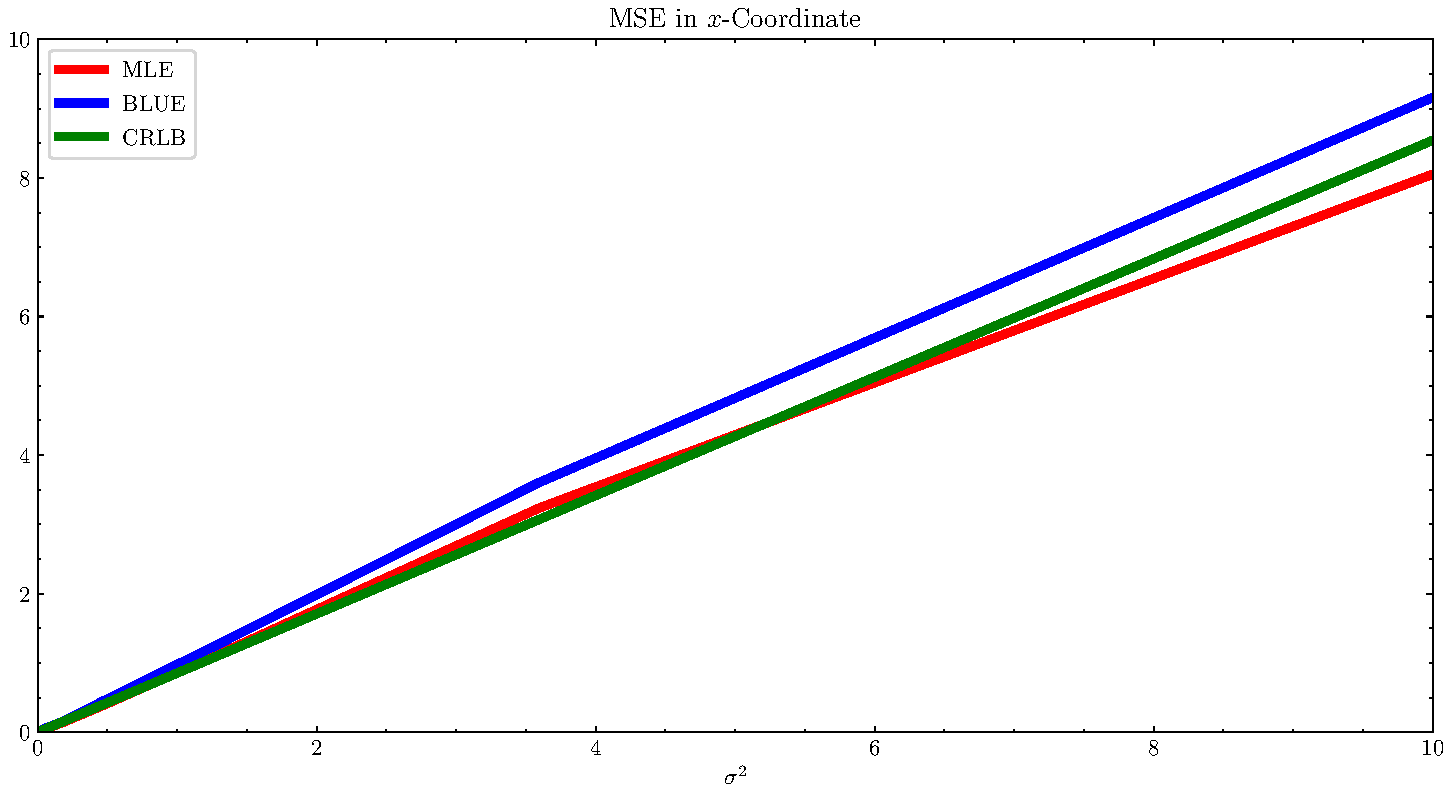
\includegraphics[width=6in]{../results/crlb_x.pdf}}
\subfigure[]{\label{fig:crlbY}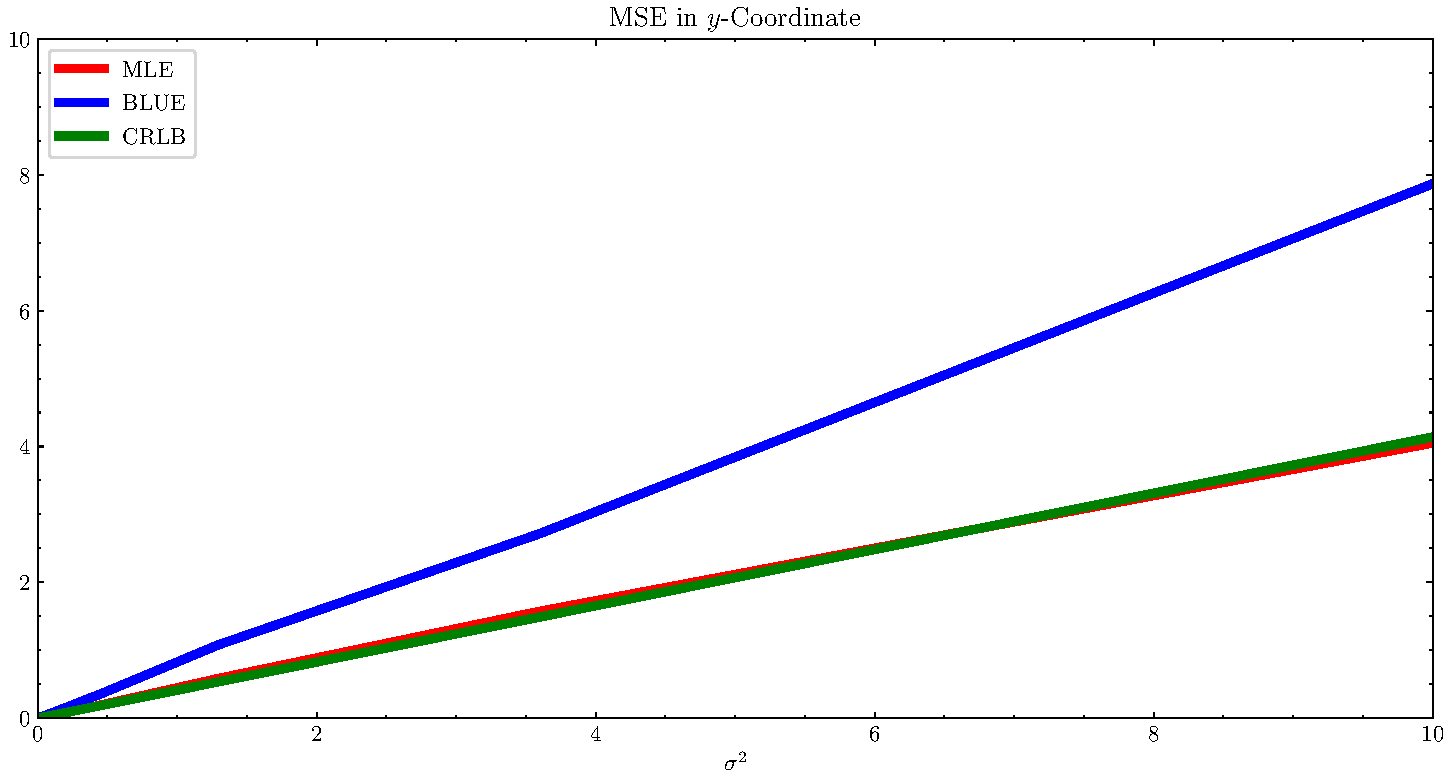
\includegraphics[width=6in]{../results/crlb_y.pdf}}
\caption{Noise analysis of TDOA localisation using MLE and BLUE estimates.}
\end{figure}

% -----------------------------------------------------------------------------------------------------------------------
% -----------------------------------------------------------------------------------------------------------------------

\appendix

\newpage
\subsection*{Scripts}
The Python3 scripts to generate all figures can be downloaded from the GitHub repository \url{https://github.com/kamath-abhijith/TDOA_Localisation}. Use \texttt{requirements.txt} to install all dependencies. Also, see the following code snippets for reference.

\newpage
\subsubsection*{Implementation of TDOA Localisation using MLE}

The relevant function to implement MLE estimate \texttt{mle\_tdoa} is in \texttt{utils.py}.
\lstinputlisting[language=Python]{../tdoa_ml.py}

% -----------------------------------------------------------------------------------------------------------------------

\subsubsection*{Implementation of TDOA Localisation using BLUE}

The relevant function to implement BLUE estimate \texttt{blue\_tdoa} is in \texttt{utils.py}.
\lstinputlisting[language=Python]{../tdoa_blue.py}

% -----------------------------------------------------------------------------------------------------------------------

\subsubsection*{Noise Analysis of TDOA Localisation using MLE and BLUE}

The relevant function to compute the CRLB \texttt{crlb\_tdoa} is in \texttt{utils.py}.
\lstinputlisting[language=Python]{../tdoa_montecarlo.py}

% -----------------------------------------------------------------------------------------------------------------------

\subsubsection*{\texttt{utils.py}}

This script contains all the relevant functions and helpers.
\lstinputlisting[language=Python]{../utils.py}

\end{document}
